% "Станет проще"

\documentclass[a4paper,12pt]{article} % тип документа

% report, book

%  Русский язык

\usepackage[T2A]{fontenc}			% кодировка
\usepackage[utf8]{inputenc}			% кодировка исходного текста
\usepackage[english,russian]{babel}	% локализация и переносы


% Математика
\usepackage{amsmath,amsfonts,amssymb,amsthm,mathtools} 
\usepackage[left=20mm, top=20mm, right=20mm, bottom=20mm, nohead, nofoot]{geometry}

% Картинки
\usepackage{graphicx}
\graphicspath{{pictures/}}
\DeclareGraphicsExtensions{.pdf,.png,.jpg}



\usepackage{wasysym}
%\documentclass[12pt]{article}
\usepackage{tikz}

%Заговолок
\author{Веприков Андрей Сергеевич}
\title{Кейс для бизнес-аналитика}
\date{}

\begin{document} % начало документа

\maketitle

\section*{Введение}

Планировщик задач - это то, без чего современному человеку невозможно обойтись в повседневной жизни. Из-за большого объема информации сложно запомнить все, для этого и нужны планировщики задач. Раньше их функцию исполняли записные книжки и ежедневники, но сейчас они уже не актуальны, когда у всех есть телефоны и компьютеры.

Как мне кажется, самое важное в нашем приложении сделать его непохожим на уже существующие планировщики задач, как например втроенные календари в IOS и Android, Google Календарь и так далее. Мы можем сделать несколько существенных отличий от этих, безусловно отличных, планировщиков задач:

\begin{enumerate}

\item[$\bullet$] Интеграция сервисов Тинькофф в наш планировщик. Это самое больше преимущество по сравнению со всеми вышеперечисленными приложениями, так как это очень удобно сразу из календаря оплатить штраф или вернуть долг другу.

\item[$\bullet$] Можно будет каждый день писать про траты пользователя за этот день. Мне кажется эта функция очень удобной, ведь будет наглядно видно, в какой день пользователь потратил больше всего денег и на что.

\item[$\bullet$] Голосовой помошник Олег может записывать какие-то события в календарь по просьбе пользователя. Сейчас, насколько я понимаю, голосовой помошник Олег работает только в приложении Тинькофф Банк, а с нашим планировщиком он сможет выполнять намного больше функций.

\item[$\bullet$] Ещё можно добавить что то типа заметок для дел, которые нужно сделать не в какой-то конкретный день, а, например, в течение недели (отдать долг, позвонить маме и т.д)

\end{enumerate}

Однако не стоит забывать о функциях, которые есть во всех планировщиках задач, которые я знаю, и без которых пользоваться нашим приложением будет попросту неудобно. Я опишу их ниже, в разделе про Функции нашего приложения.

\section*{Список user-story}

Наш пользователь захочет добавить какое-то событие в календарь, чтобы не забыть о нём и в будущем правильно составить своё расписание на этот день. Он может записать что-то в заметки, чтобы не забыть сделать это в течении недели или месяца.

Пользователь захочет добавлять задачи в избранное, разбивать их на категории, делать какие-то задачи повторяющимися, добавлять других пользователей к своей задаче, делиться ею в интернете, чтобы ему было удобнее.

Пользователь захочет получать уведомления о предстоящих задачах, чтобы о них не забыть.

Пользователь захочет получать информацию о том, как можно решить его задачу с помощью сервисов Тинькофф, чтобы ему было легко и быстро решать свои дела. 

Можно придумать ещё много вариантов user-story, но я лучше опишу все основные функции нашего приложения.

\section*{Функции нашего приложения}

\begin{enumerate}

\item[$\bullet$] Добавить задачу в календарь или в заметки

\item[$\bullet$] Добавлять задачи в избранное, разбивать их на категории (можно, например, делать для каждой категории разный цвет)

\item[$\bullet$] Возможность подключить других пользователей к своей задаче, возможность поделиться ей через интернет

\item[$\bullet$] Создание задач, повторяющихся с какой-то периодичностью (например: неделя или месяц)

\item[$\bullet$] Возможность добавить список продуктов или коротких дел в заметки

\item[$\bullet$] Уведомления о предстоящих задачах

\item[$\bullet$] Изменение темы со светлой на тёмную

\item[$\bullet$] Возможность перенести своё расписание из других планировщиков или календарей

\item[$\bullet$] Подключение голосового помошника Олега

\end{enumerate}

Важную роль в нашем приложении будет играть интеграция сервисов Тинькофф, поэтому для каждого сервиса опишем, как можно использовать их с нашим планировщиком:

\subsection*{Интеграция сервисов Тинькофф} 

\begin{enumerate}

\item[\textbf{1)}] \textbf{Тинькофф Банк}

Можно будет писать о тратах пользователя за день, также можно будет в конце каждого месяца делать небольшой отчёт о потраченных средствах. Если пользователь запишет в заметки: <<Отдать долг 100 рублей Ивану Иванову>>, то по нажатию на эту запись происходит переход в приложение банка на страницу перевода денег, где сразу написана сумма и получатель (если сумма или получатель не написан в заметке, то эти поля будут пустыми).

\item[\textbf{2)}] \textbf{Кино, Рестораны и Театры}

Если пользователь записал в календаре поход в кино, ресторан или театр, то можно предложить пользователю ссылку на соответствующий сервис, где он может купить билеты или заказать столик.

\item[\textbf{3)}] \textbf{Цветы, Косметика и Красота}

Представим ситуацию, скоро день матери, это будет отмечено в нашем календаре и эти сервисы будут показаны нашему пользователю как возможные варианты подарков. Кроме дня матери можно, например, ввести дату дня рождения друга или подруги и так далее.

\item[\textbf{4)}] \textbf{Шопинг}

Как вариант, можно каждое первое воскресенье месяца предлагать пользователю сходить по магазинам. Разумеется дату можно будет менять.

\item[\textbf{5)}] \textbf{Спорт}

Допустим, мы знаем, что наш пользователь любит футбол (об этом можно спросить в самом начале работы с приложением), тогда мы можем перед какими-то важными матчами по футболу в городе пользователя показывать ему ссылку на покупку билетов в этом приложении.

\item[\textbf{6)}] \textbf{Товары}

Если пользователь создал список покупок в заметках, то мы будем предлагать не самому идти в магазин, а заказать продуты онлайн через сервис Товары, также можно по списку товаров составить примерную корзину, чтобы пользователь не искал все продукты, которые он вбил в список. 

\end{enumerate}

Это вариант интеграции некоторых сервисов Тинькофф в наш планировщик задач, они, конечно, не покрывают всех потребностей пользователя, но ему безусловно будет намного легче, если они все будут внедрены в наше приложение.

Разумеется, каждую из этих функций можно будет отключить, если конкретному пользователю они не нужны.

\section*{Возможный вариант интерфейса пользователя}

\begin{figure}[h!]
\center
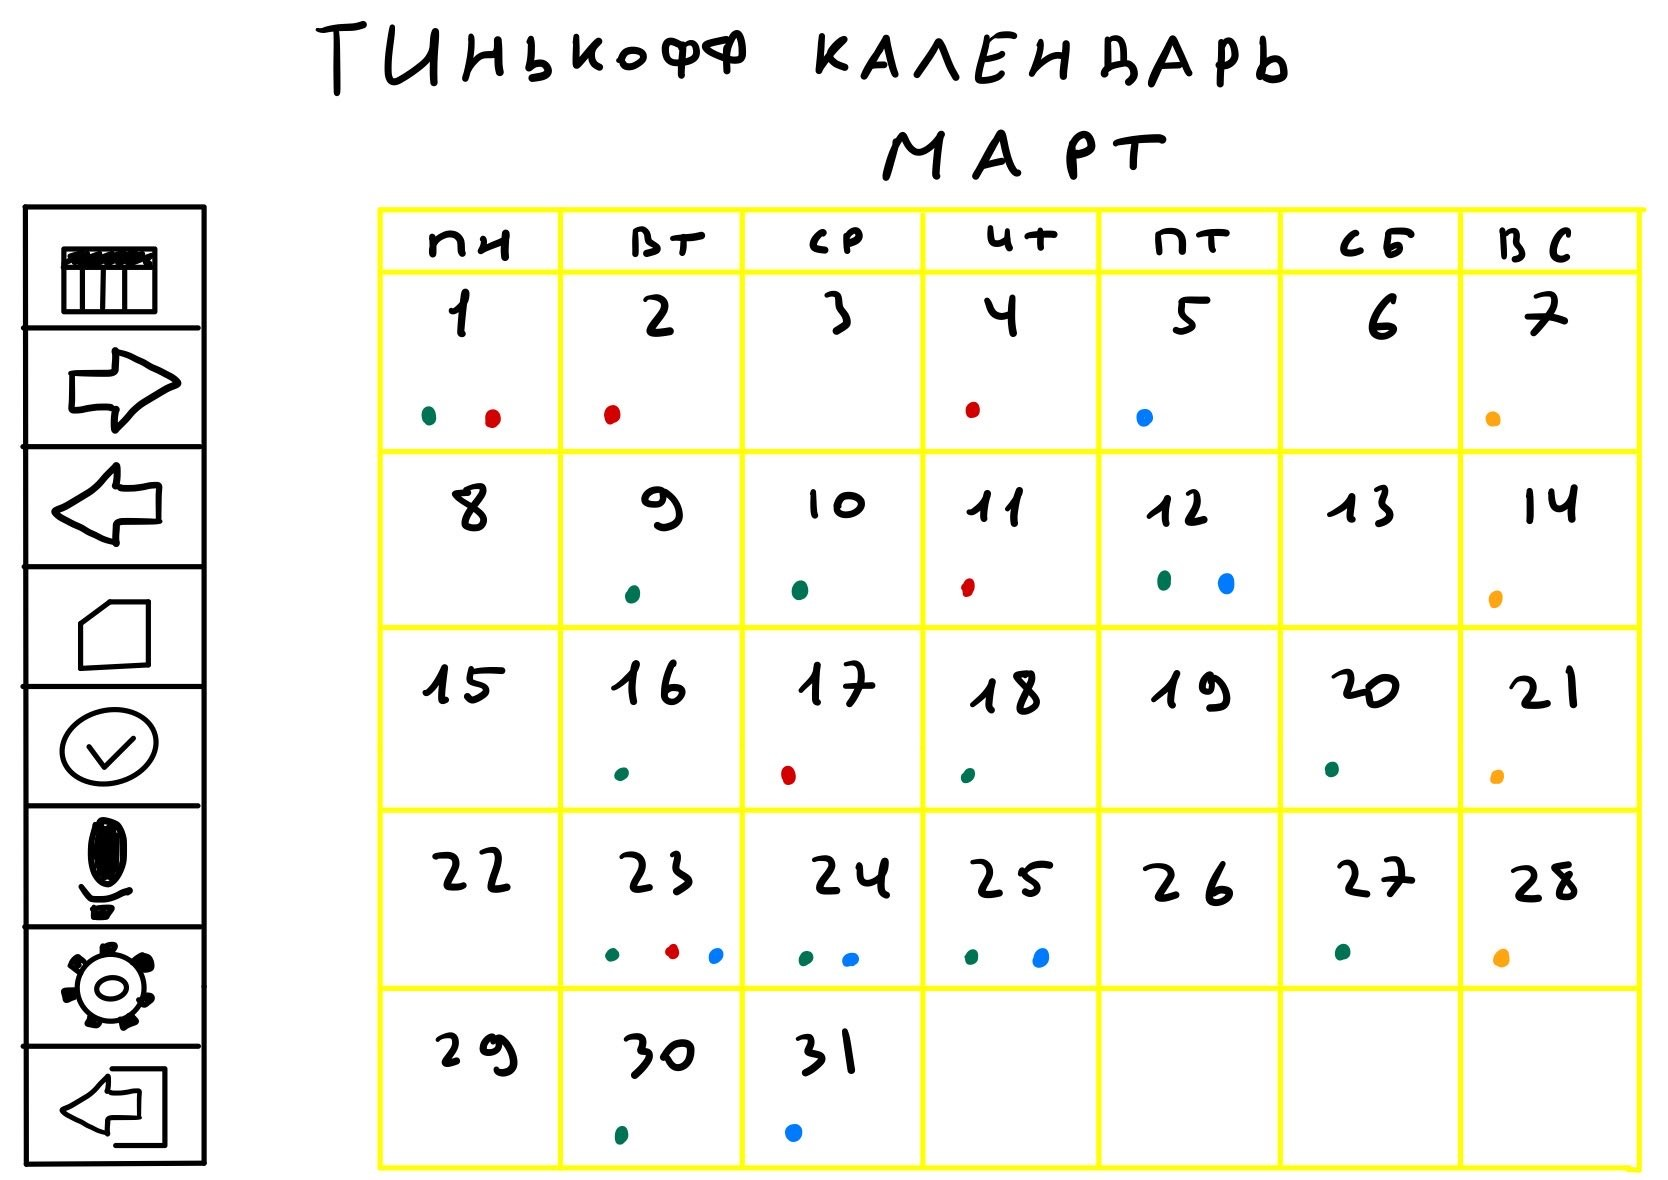
\includegraphics[scale=0.2]{Interface}
\end{figure}

Так как я не супер художник, давайте поясню что на картинке что означает. Слева расположены иконки: 1 - это переход к заметкам; 2, 3 - это переход на 1 месяц вперед или назад; 4, 5 - это шаблоны событий в календаре и заметках соответственно; 6 - это голосовой помошник Олег; 7 - это настройки; 8 - это выход из аккаунта.

Справа расположен сам календарь, на каждую дату можно нажать и перейти конкретно в этот день, чтобы добавить туда событие. Разноцветные точки в некоторых датах - это уже добавленные события, каждый цвет соответствует своей категории событий.

Разумеется, это сырой вариант интерфейса, но примерную логику работы приложения я показал на этом примере.

\newpage

\section*{Схема бизнес-процесса в рамках какой-либо user-story}

Допустим, какой-то пользователь захотел пойти в кино 20 марта. Он заходит в наше приложение, нажимает на дату 20, там ему открывается 20 число, он нажимает на кнопку <<+>> (добавить событие), и ему сразу выдаются его варианты шаблонов. Допустим, у него нет шаблона на поход в кино, он добавляет время, допустим, 18:00 - 21:00, называет событие <<Поход в кино с Пашей>> и добавляет это событие в категорию <<Развлечения>>, когда он создал это событие ему показывается подсказка, что можно купить билеты в кино через сервис Тинькофф Кино, он нажимает на эту подсказку, переходит на сервис и покупает там билеты, когда он купил их подсказка пропадает.

\section*{Возможный QPI}

\begin{enumerate}

\item[$\bullet$] Количество загрузок приложения

\item[$\bullet$] Среднее количество записей событий у всех пользователей

\item[$\bullet$] Количество переходов по подсказкам для событий (или можно отношение переходов ко всем возможным переходам)

\item[$\bullet$] Среднее время использования приложения

\item[$\bullet$] Деньги, которые компания выручит за все переходы по подсказкам.

\end{enumerate}

\section*{Вывод}

Как мне кажется, планировщик от Тинькофф может стать очень популярным приложением, так как оно будет покрывать многие потребности своих пользователей. Но для успешной работы приложения необходимо интегрировать остальные сервисы Тинькофф, чтобы пользователям было максимально удобно. Сейчас у многих компаний есть свой планировщик задач, например у Google, и мне кажется компания Тинькофф не должна оставаться в стороне.

\end{document}